\section{Experiments}
\label{sec:experiments}
\begin{figure*}[t]
\centering
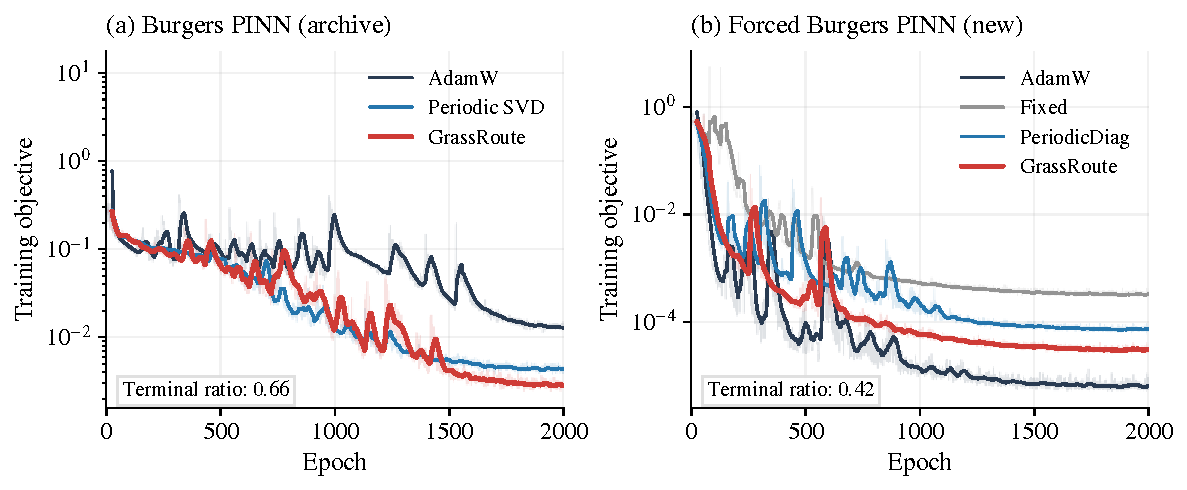
\includegraphics[width=\linewidth]{figures/fig_core_loss.pdf}
\caption{Core loss trajectories supporting the scientific-learning advantage,
with the competing outcomes retained. All panels show 2000 stored epochs:
faint lines are the raw objectives, solid lines are 25-epoch trailing means.
``Terminal ratio'' is the ratio of the final-100-epoch mean losses,
GrassRoute / periodic comparator; below one favors GrassRoute.
(a) Three archived Burgers trajectories: GrassRoute ends below AdamW and
periodic SVD. These stored curves are distinct from the tuned scalar summaries
in Table~\ref{tab:archive}; the objective is the archived residual-plus-initial-condition
loss, with its boundary-condition specification in Appendix~\ref{app:audit}.
(b) Independent validation-selected forced Burgers with corrected periodic
moment transport. GrassRoute improves on the matched-state periodic run;
AdamW remains stronger. The Poisson loss control appears in
Figure~\ref{fig:poisson-loss-control}. No best epoch is selected and no
cross-protocol loss magnitude is pooled. Seed 42 only.}
\label{fig:core-loss}
\end{figure*}
We distinguish archived results from a new validation-selected extension. They use different state-transport versions and, for several tasks, different data/model protocols. Their numerical endpoints are not pooled. All formal runs use seed 42, as specified by the proposal. The extension includes the official SubTrack++ optimizer; the historical B6 was an unofficial geodesic surrogate.

Figure~\ref{fig:core-loss} makes the positive loss evidence explicit rather
than inferring it from endpoint tables. The stored archived GrassRoute run
ends at $2.978\times10^{-3}$, compared with $1.368\times10^{-2}$ for AdamW
and $3.881\times10^{-3}$ for periodic SVD, with every intermediate epoch
retained. The independent follow-up panel shows where that advantage
transfers and where the strongest competing method remains better. Lower
training objective is not equated with lower held-out solution error.

\subsection{Scientific-learning and graph evidence}
The archived Burgers PINN supplies the clearest joint training-loss--state
observation: its tuned best loss is $1.97\times10^{-3}$ versus AdamW's
$1.10\times10^{-2}$ and periodic SVD's $3.27\times10^{-3}$, with 84.1\%
less persistent optimizer state. Figure~\ref{fig:core-loss} separately shows
all epochs of the stored trajectories. The archive reports a 1.78$\times$
step cost, and its residual-plus-initial-condition objective omits an explicit
spatial boundary penalty. This supports a scoped training-loss--memory result,
not a claim of superior physical solution accuracy. All recovered endpoints,
including the unsuccessful task families, remain in
Appendix~\ref{app:full-results}.

In the independent expanded-search Cora comparison, GrassRoute obtains
78.6\% test accuracy versus AdamW's 77.5\%, corrected periodic routing's
77.7\%, and official SubTrack++'s 77.3\%. Its persistent optimizer state is
207,368 bytes versus AdamW's 2,950,224, a 93.0\% reduction. SGD reaches
79.7\% with 1,475,100 bytes; thus GrassRoute supplies a favorable
accuracy--state operating point rather than the highest accuracy across
all six methods. The comparison uses the same nine-candidate validation budget
and fresh 1000-epoch formal runs (Table~\ref{tab:graph-strength}).

\input{figures/focused_gcn_main}
With the seed-42 Cora GraphSAGE hyperparameters frozen, three new initializations give mean final test accuracy 76.90\% for GrassRoute, 77.63\% for AdamW and 79.23\% for SGD-M. GrassRoute exceeds AdamW in 1/3 paired seeds. Corrected periodic SVD records 78.10\%, 78.60\% on its completed seeds and a retained numerical failure on the other. The favorable seed-42 accuracy--state observation is therefore not consistent across these new initializations; all endpoints and the failure appear in Table~\ref{tab:focused-cora-replication}.\par


\input{figures/revision_main_positive}

\subsection{Evaluation scope and complete reporting}
We distinguish strict primary-metric gains from accuracy--memory trade-offs.
The original proposal extension specified 27 representative configurations
and six methods, selected by validation before 1000 or 2000 complete formal
epochs. After 117 of 162 task--method runs finished, we stopped its remaining
high-cost image and continual-learning queue and redirected computation to
focused exploratory checks. This scope decision followed inspection of
completed results and cannot support a claim of prospective full coverage.
The original outcome matrix retains every completed, unfavorable and pending
cell in Appendix~\ref{app:full-results}. A controlled drifting-regression
study and a second Cora architecture are reported separately in
Appendix~\ref{app:focused-followup}. New public-data domains use another
frozen protocol below. All experiments use seed 42;
finite tuning budgets and one-seed observations do not imply statistical
significance or a universal optimizer ranking.

\subsection{Testing the mathematical mechanisms}
The controlled diagnostics isolate angle dependence at a fixed eigengap, QR/exponential discrepancy, and tracking under known population drift. They use full covariance spectra and actual oracle subspaces, with 600 random landscape checks and a 27-setting tracking bed. A separate neighboring-data experiment replaces one CIFAR-100 image while training a linear probe on frozen random ResNet features for 1000 epochs. It measures parameter and bounded-loss sensitivity, rather than equating a train--test gap with uniform stability. These auxiliary tests are not counted as additional end-to-end task-family wins. Their protocols and diagnostic tables appear in Appendix~\ref{app:audit}.

The complete mechanism grids, resource tables and expanded-search follow-ups are reported in Appendix~\ref{sec:strength-followup}.
